\documentclass[12pt]{article}

\input{../../Latex_Common/skinnerr_latex_preamble_asen5417.tex}

%%
%% DOCUMENT START
%%

\begin{document}

\pagestyle{fancyplain}
\lhead{}
\chead{}
\rhead{}
\lfoot{ASEN 5417: Homework 2}
\cfoot{\thepage}
\rfoot{Ryan Skinner}

\noindent
{\Large Homework 2}
\hfill
{\large Ryan Skinner}
\\[0.5ex]
{\large ASEN 5417: Numerical Methods}
\hfill
{\large Due 2015/09/17}\\
\hrule
\vspace{6pt}

\section{Introduction}

We solve the following problems to better understand numerical techniques for solving ordinary differential equations. As will be described in the methods section, our tools primarily consist of second- and fourth-order Runge-Kutta methods, and Euler stability analysis.

\subsection{Problem 1}

Equations of motion for a rocket's vertical speed $v$ can be written as
\begin{equation}
(m_c + m_p) \frac{dv}{dt} = -(m_c + m_p) g + \dot{m}_p v_e - \tfrac{1}{2} \rho v \norm{v} A C_D
,
\label{eq:rocket}
\end{equation}
where $z$ is the vertical coordinate, $v = dz/dt$ is the vertical speed, and
\begin{equation*}
\begin{aligned}
m_c &= 51.02 \text{ kg} &&\text{(rocket casing mass)} \\
g &= 9.8 \text{ m/s}^2 &&\text{(gravitational acceleration)} \\
\rho &= 1.23 \text{ kg/m}^3 &&\text{(air density)} \\
A &= 0.1 \text{ m}^2 &&\text{(maximum cross-sectional area)} \\
v_e &= 360 \text{ m/s} &&\text{(exhaust speed)} \\
C_D &= 0.15 &&\text{(drag coefficient)} \\
m_{p0} &= 102.04 \text{ kg} &&\text{(initial propellant mass)}
.
\end{aligned}
\end{equation*}
Furthermore, the instantaneous propellant mass at time $t$ is given by
\begin{equation}
m_p(t) = m_{p0} - \int_0^t \dot{m}_p dt
,
\end{equation}
and the time-varying burn rate is
\begin{equation}
\dot{m}_p =
\frac{m_{p0}}{4}
\cdot
\begin{cases}
t     & 0 \le t \le 1 \\
1     & 1 \le t \le 4 \\
5 - t & 4 \le t \le 5 \\
0     & 5 \le t
.
\end{cases}
\end{equation}

Use a second-order Runge-Kutta (RK2) integrator with $\Delta t = 0.1 \text{ s}$ to plot $z(t)$ and $v(t)$. Use these plots to find the maximum speed, and the height and time at which it is reached; the maximum height, and the time at which it is reached; and the time and velocity when the rocket hits the ground. Check these results with those obtained from \textsc{Matlab}'s \lstinline|ode45| solver.

This problem is fairly straight-forward. An RK2 scheme is relatively easy to implement, but we will need to be careful when accounting for the time-dependence of $m_p$. Furthermore, though it is not stated in the problem, when $m_p$ reaches zero, the thrust term involving the exhaust speed $v_e$ in \eqref{eq:rocket} needs to ``turn off.''

\subsection{Problem 2}

Consider the stream function for a two-dimensional jet in self-similar form, which can be written as
\begin{equation}
f''(\eta) + f(\eta) f'(\eta) = 0 ,\qquad
f(0) = 0 ,\qquad
f'(0) = 1
.
\end{equation}
The velocities in the jet can be obtained via
\begin{equation}
\frac{U}{U_0} = f'(\eta) ,\qquad
\frac{V}{U_0} = \eta f'(\eta) - \tfrac{1}{2} f(\eta)
.
\end{equation}
Using numerical integration for $0 \le \eta \le 4$, with a step size of $\Delta \eta = 0.05$, plot the quantities $U/U_0$, $V/V_0$, and $f$ as functions of $\eta$. Perform this analysis with both the second- and fourth-order Runge-Kutta methods, and compare their performance. Both solutions may be compared to those obtained from the best-fit expression
\begin{equation}
f(\eta) = \exp(-0.682 \eta^2)
.
\end{equation}

\subsection{Problem 3}

Show that the equation
\begin{equation}
y'' = -\frac{19}{4} y - 10 y' ,\qquad
y(0) = -9 ,\qquad
y'(0) = 0
\end{equation}
is moderately stiff. Use Euler stability analysis to estimate the largest step size $h_\tmax$ for which the Runge-Kutta method will be stable. Then confirm this estimate by computing $y$ using the fourth-order Runge-Kutta method with $h = \{ \tfrac{1}{2} h_\tmax, 2 h_\tmax\}$. Compare these solutions with the analytical solution.

\section{Methodology}

\subsection{Problem 1}

We first re-write the system of equations governing rocket altitude as
\begin{equation}
\begin{aligned}
\frac{dz}{dt} &= f(t,v) &&= v
\\
\frac{dv}{dt} &= g(t,v) &&= \underbrace{-g + T \frac{\dot{m}_p v_e}{(m_c + m_p)}}_{\alpha(t)} + \underbrace{\frac{- \rho A C_D}{2 (m_c + m_p)}}_{\beta(t)} v \norm{v}
,
\end{aligned}
\label{eq:rocket_rewritten}
\end{equation}
where $\alpha$ and $\beta$ are constants that directly depend only on time, and $T$ toggles the thrust term on and off based on whether the rocket is still burning propellant.

Given the initial values of our variables at $t=0$, the second-order Runge-Kutta method allows us to integrate the system of equations \eqref{eq:rocket_rewritten} with respect to time using a time step $h$. At a given time $t_n$, the velocity and position at the next time step, $v_{n+1}$ and $z_{n+1}$, can be approximated by applying the following formulae to each successive time step: calculating
\begin{equation}
\begin{aligned}
k_1 &= h f(t_n,v_n) &&= h v_n
\\
l_1 &= h g(t_n,v_n) &&= h \left[ \alpha(t_n) + \beta(t_n) v_n \norm{v_n} \right]
\\
k_2 &= h f(t_n + h/2, v_n + k_1 / 2) &&= h \left[ v_n + k_1/2\right]
\\
l_2 &= h g(t_n + h/2, v_n + l_1 / 2) &&= h \left[ \alpha(t_n + h/2) + \beta(t_n + h/2) (v_n + l_1 / 2) \norm{v_n + l_1 / 2} \right]
\end{aligned}
\end{equation}
and then updating the next step's values of $z$ and $v$ as
\begin{equation}
\begin{aligned}
z_{n+1} &= z_n + k_2
\\
v_{n+1} &= v_n + l_2
.
\end{aligned}
\end{equation}

\section{Results}

\subsection{Problem 1}

Plots of the velocity and altitude time histories are presented in \figref{fig:rocket_plots}. Statistics on notable flight events are shown in Table~\ref{tbl:rocket}.

\begin{figure}[t]
\begin{center}
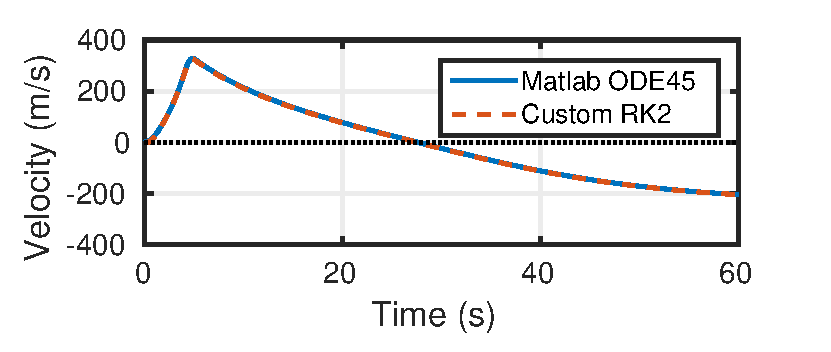
\includegraphics[width=0.49\textwidth]{rocket_velocity.eps}
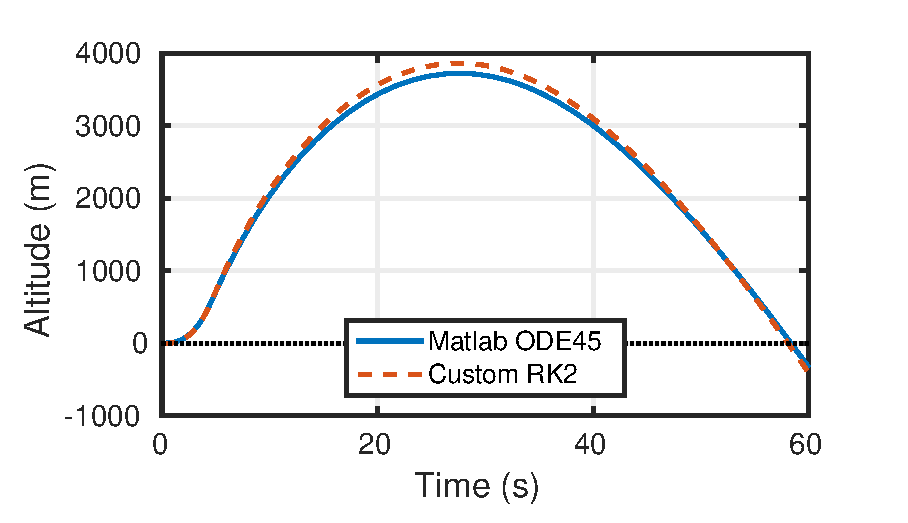
\includegraphics[width=0.49\textwidth]{rocket_altitude.eps}
\\[6pt]
\caption{Comparison of our own 2\nd-order Runge-Kutta scheme to \textsc{Matlab}'s \lstinline|ode45| solver, for the rocket velocity and altitude.}
\label{fig:rocket_plots}
\end{center}
\end{figure}

\begin{table}[t]
\centering
\begin{tabular}{llllllll}
\toprule
Integrator   & \multicolumn{3}{c}{Max Velocity} & \multicolumn{2}{c}{Max Altitude} & \multicolumn{2}{c}{Crash} \\
\midrule
~            & Time & Velocity & Altitude       & Time         & Altitude & Time  & Velocity \\
Custom RK2   & 4.80 & 325.10   & 649.86         & 27.50        & 3850.40  & 57.98 & -199.65  \\
\textsc{Matlab} \lstinline|ode45| & 4.67 & 327.01   & 597.32         & 27.36        & 3726.67  & 58.40 & -200.27 \\
\bottomrule
\end{tabular}
\\[6pt]
\caption{Comparison of notable flight events between integration methods.}
\label{tbl:rocket}
\end{table}

\section{Discussion}

\section{References}

No external references were used other than the course notes for this assignment.

\section*{Appendix: MATLAB Code}
The following code listings generate all figures presented in this homework assignment.

\includecode{Problem_1.m}



%%
%% DOCUMENT END
%%
\end{document}
